\documentclass{article}
\usepackage[utf8]{inputenc}
\usepackage{minted}
\usepackage[a4paper, top=1in, left=0.5in, right=0.5in, bottom=1in]{geometry}
\usepackage{fancyhdr}
\usepackage{tikz}
\usepackage{pgfplots}
\usepackage{amssymb}

\setcounter{secnumdepth}{5}
\setcounter{tocdepth}{5}
\pgfkeys{/pgf/number format/.cd,1000 sep={\,}}

\pagestyle{fancy}
\chead{\Large{Reference document, Nikolay Budin}}
\lhead{Generated \today \\
\textcolor{red}{1 error}, \textcolor{orange}{4 warnings}
}
\rhead{ITMO University}

\begin{document}
\tableofcontents

\newpage

\section{Data structures}
\subsection{Fenwick tree}
\inputminted[mathescape, breaklines, tabsize=4, frame=lines, linenos=true]{c++}{./data-structures/fenwick-tree/fenwick-tree.cpp}
\textcolor{orange}{\textbf{Warning:} No tests}
\section{Graphs}
\subsection{Hungarian algorithm}
\inputminted[mathescape, breaklines, tabsize=4, frame=lines, linenos=true]{c++}{./graphs/hungarian_algorithm/hungarian_algorithm.cpp}
\textcolor{orange}{\textbf{Warning:} No tests}
\section{String algorithms}
\subsection{Manacher algorithm (longest palindrome for every center)}
\inputminted[mathescape, breaklines, tabsize=4, frame=lines, linenos=true]{c++}{./strings/manacher/manacher.cpp}
\textcolor{violet}{\checkmark Tests passed}
\begin{center}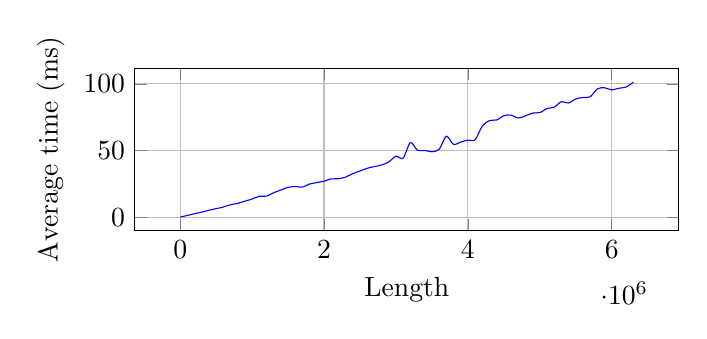
\begin{tikzpicture}
	\begin{axis}[
		xlabel=Length,
		ylabel=Average time (ms),
		grid=major,
		scaled y ticks=false,
		y tick label style={/pgf/number format/fixed},
		width=0.7\textwidth,
		height=0.3\textwidth]
	\addplot[color=blue, smooth] coordinates {
		(1, 0.00013)
(100001, 1.24465)
(200001, 2.52502)
(300001, 3.69951)
(400001, 5.12818)
(500001, 6.33875)
(600001, 7.53767)
(700001, 9.32370)
(800001, 10.32313)
(900001, 11.96350)
(1000001, 13.53895)
(1100001, 15.63436)
(1200001, 15.70784)
(1300001, 18.29608)
(1400001, 20.35170)
(1500001, 22.31783)
(1600001, 22.96069)
(1700001, 22.50002)
(1800001, 24.84532)
(1900001, 25.90111)
(2000001, 26.96264)
(2100001, 28.70058)
(2200001, 28.75973)
(2300001, 30.02441)
(2400001, 32.63076)
(2500001, 34.59773)
(2600001, 36.61562)
(2700001, 37.90908)
(2800001, 39.07795)
(2900001, 41.41936)
(3000001, 45.68448)
(3100001, 44.21825)
(3200001, 55.91109)
(3300001, 50.12750)
(3400001, 50.04995)
(3500001, 49.06843)
(3600001, 50.84135)
(3700001, 60.72149)
(3800001, 54.58675)
(3900001, 56.32501)
(4000001, 57.82212)
(4100001, 57.98866)
(4200001, 68.32811)
(4300001, 72.43886)
(4400001, 72.90059)
(4500001, 76.10515)
(4600001, 76.55721)
(4700001, 74.39213)
(4800001, 75.99793)
(4900001, 78.10147)
(5000001, 78.46419)
(5100001, 81.47732)
(5200001, 82.53965)
(5300001, 86.62287)
(5400001, 85.59356)
(5500001, 88.74211)
(5600001, 89.72947)
(5700001, 90.32142)
(5800001, 96.25297)
(5900001, 97.06376)
(6000001, 95.47867)
(6100001, 96.75415)
(6200001, 97.62596)
(6300001, 101.27108)

	};
	\end{axis}
\end{tikzpicture}\end{center}\subsection{Prefix function}
\inputminted[mathescape, breaklines, tabsize=4, frame=lines, linenos=true]{c++}{./strings/pref_function/pref_function.cpp}
\textcolor{violet}{\checkmark Tests passed}
\begin{center}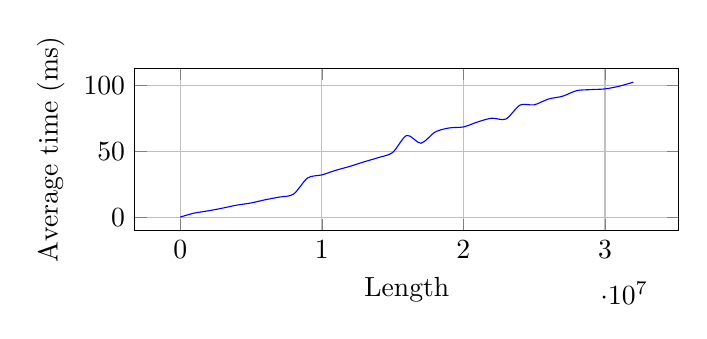
\begin{tikzpicture}
	\begin{axis}[
		xlabel=Length,
		ylabel=Average time (ms),
		grid=major,
		scaled y ticks=false,
		y tick label style={/pgf/number format/fixed},
		width=0.7\textwidth,
		height=0.3\textwidth]
	\addplot[color=blue, smooth] coordinates {
		(1, 0.00004)
(1000001, 3.04782)
(2000001, 4.79016)
(3000001, 6.82951)
(4000001, 9.09451)
(5000001, 10.70848)
(6000001, 13.16447)
(7000001, 15.19880)
(8000001, 17.39937)
(9000001, 29.70328)
(10000001, 32.05185)
(11000001, 35.57767)
(12000001, 38.58729)
(13000001, 42.00489)
(14000001, 45.22427)
(15000001, 49.05340)
(16000001, 62.04580)
(17000001, 56.10121)
(18000001, 64.61456)
(19000001, 67.72562)
(20000001, 68.48828)
(21000001, 72.24345)
(22000001, 75.13236)
(23000001, 74.47957)
(24000001, 85.12094)
(25000001, 85.28631)
(26000001, 89.67687)
(27000001, 91.81448)
(28000001, 96.06844)
(29000001, 96.84945)
(30000001, 97.39997)
(31000001, 99.42471)
(32000001, 102.50109)

	};
	\end{axis}
\end{tikzpicture}\end{center}\subsection{Suffix structures}
\subsubsection{Suffix array}
\inputminted[mathescape, breaklines, tabsize=4, frame=lines, linenos=true]{c++}{./strings/suff_algorithms/suff_array/suff_array.cpp}
\textcolor{violet}{\checkmark Tests passed}
\begin{center}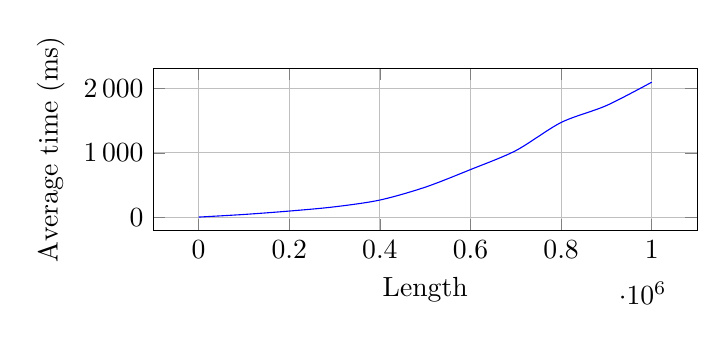
\begin{tikzpicture}
	\begin{axis}[
		xlabel=Length,
		ylabel=Average time (ms),
		grid=major,
		scaled y ticks=false,
		y tick label style={/pgf/number format/fixed},
		width=0.7\textwidth,
		height=0.3\textwidth]
	\addplot[color=blue, smooth] coordinates {
		(1, 0.00047)
(100001, 40.81160)
(200001, 93.77239)
(300001, 159.74959)
(400001, 265.18201)
(500001, 465.04838)
(600001, 739.25857)
(700001, 1034.47205)
(800001, 1472.12715)
(900001, 1735.42908)
(1000000, 2099.11813)

	};
	\end{axis}
\end{tikzpicture}\end{center}\section{FFT}
\subsection{FFT by modulo}
\inputminted[mathescape, breaklines, tabsize=4, frame=lines, linenos=true]{c++}{./fft/mod/mod_fft.cpp}
\textcolor{red}{\textbf{Error:} Compilation error while compiling test}
\subsection{FFT in complex numbers}
\textcolor{orange}{\textbf{Warning:} Leaf directory without any information}
\section{Convex hull trick}
\subsection{Arbitrary order of lines}
\inputminted[mathescape, breaklines, tabsize=4, frame=lines, linenos=true]{c++}{./convex-hull-trick/full/full_cht.cpp}
\textcolor{orange}{\textbf{Warning:} No tests}


\end{document}
